\documentclass[tikz,border=5mm,12pt]{standalone}
\usepackage[fontsize=16pt]{fontsize}
\usetikzlibrary{arrows.meta}

\newcommand\texty{-18mm}
\newcommand\arrowtipscale{1.5}

\begin{document}
  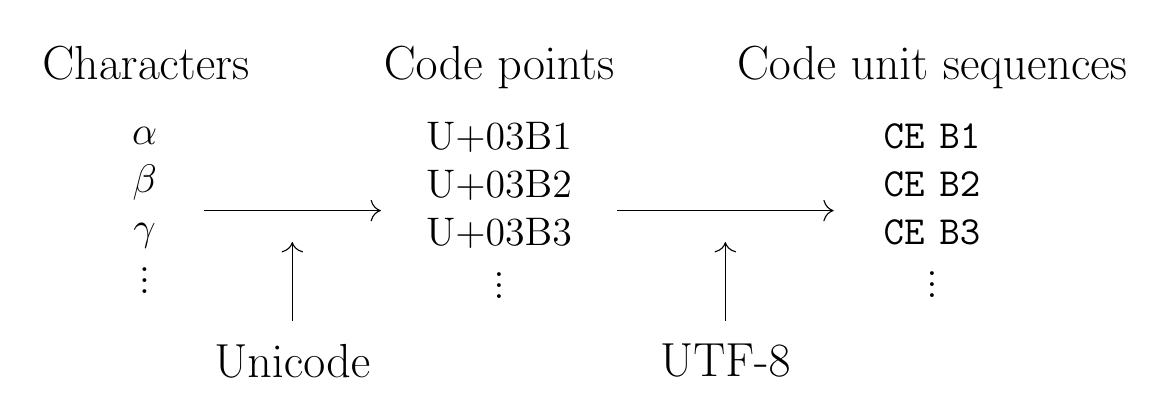
\begin{tikzpicture}
    \node[text width=26mm,align=center] at (0,0) {Characters\strut};
    \node[text width=26mm,text centered] at (0,\texty) {\small
      $\alpha$ \\
      $\beta$ \\
      $\gamma$ \\
      $\vdots$};

    \node[text width=30mm,align=center] at (45mm,0) {Code points\strut};
    \node[text width=30mm,text centered] at (45mm,\texty) {\small
      U+03B1 \\
      U+03B2 \\
      U+03B3 \\
      $\vdots$};

    \node[text width=50mm,align=center] at (100mm,0) {Code unit sequences\strut};
    \node[text width=50mm,align=center] at (100mm,\texty) {\small
      \texttt{CE B1} \\
      \texttt{CE B2} \\
      \texttt{CE B3} \\
      $\vdots$};

    \draw[-{>[scale=\arrowtipscale]}] (7.5mm,\texty) -- (30mm,\texty) coordinate[midway] (C1);
    \draw[-{>[scale=\arrowtipscale]}] (60mm,\texty) -- (87.5mm,\texty) coordinate[midway] (C2);

    \draw[{<[scale=\arrowtipscale]}-] (C1)+(0,-4mm) -- ++(0,-14mm) node[anchor=north,yshift=-1mm] {Unicode};
    \draw[{<[scale=\arrowtipscale]}-] (C2)+(0,-4mm) -- ++(0,-14mm) node[anchor=north,yshift=-1mm] {UTF-8};
  \end{tikzpicture}
\end{document}
